\section{问题分析}
数据同化的目标是在动力模型预测与带噪观测之间建立平衡，恢复尽可能接近真实状态的分析场。对于 $40$ 维 Lorenz96 系统，经典 LETKF 已具备较强的稳定性和工程实用性\cite{hunt2007letkf}，但赛题要求方案必须包含真实量子模块，并满足量子比特数不超过 $30$、代码可复现、结果可提交等限制。

基于这些约束，直接构造全量子 4D-Var 或整体量子滤波器并不现实。原因在于：一是状态维度高，难以整体编码；二是量子线路深度与资源成本难以控制；三是完全替代经典同化器会显著削弱稳定性。因此，本项目的核心问题不是“是否使用量子方法”，而是“量子信息应作用于同化流程的哪个层次，才能既合理又稳定”。

就研究定位而言，现有相关路线大致可以分为四类。第一类是经典 LETKF 与局地加权/局地化路线，重点在于通过局地观测子集和先验距离结构保持更新稳定\cite{hunt2007letkf}；第二类是量子核与量子特征映射路线，重点在于利用量子态重叠刻画样本之间的非平凡相似性\cite{yin2025photonicqkernel,saez2025qkernel,altmann2025qgk}；第三类是量子增强的动力系统建模或外层搜索路线，量子模块通常负责提供外部表征或搜索能力，而不直接进入同化公式内部\cite{felix2024reservoir}；第四类是量子滤波或量子同化的更激进路线，试图让量子模块主导状态估计过程\cite{kotsuki2024qda,giannakis2022operator}. 本文与这些路线的关系是：保留第一类的经典稳定骨架，吸收第二类的相似度表达能力，但不采用第三类仅做外层增强的角色定位，也不走第四类整体替代的高风险路线。

因此，本文的出发点不是泛泛地“设计一个量子算法”，而是更具体地问：经典同化器中哪些量仍然缺乏结构信息，且这些结构信息恰好可以由量子相似度提供。进一步分析可以看到，经典 LETKF 的强项在于更新稳定、数值可控；其潜在不足则在于局地权重通常依赖预设距离先验，难以自适应地区分“哪些观测与当前状态窗口更匹配”。量子核文献表明，量子态重叠可以在浅层线路上提供不同于经典核函数的相似度结构\cite{yin2025photonicqkernel,saez2025qkernel}。这正是量子模块最可能发挥作用的地方。换句话说，量子信息在本任务中的价值，并不体现在替代经典主骨架，而更可能体现在补充经典方法缺少的局地几何结构信息。

\begin{figure}[htbp]
\centering
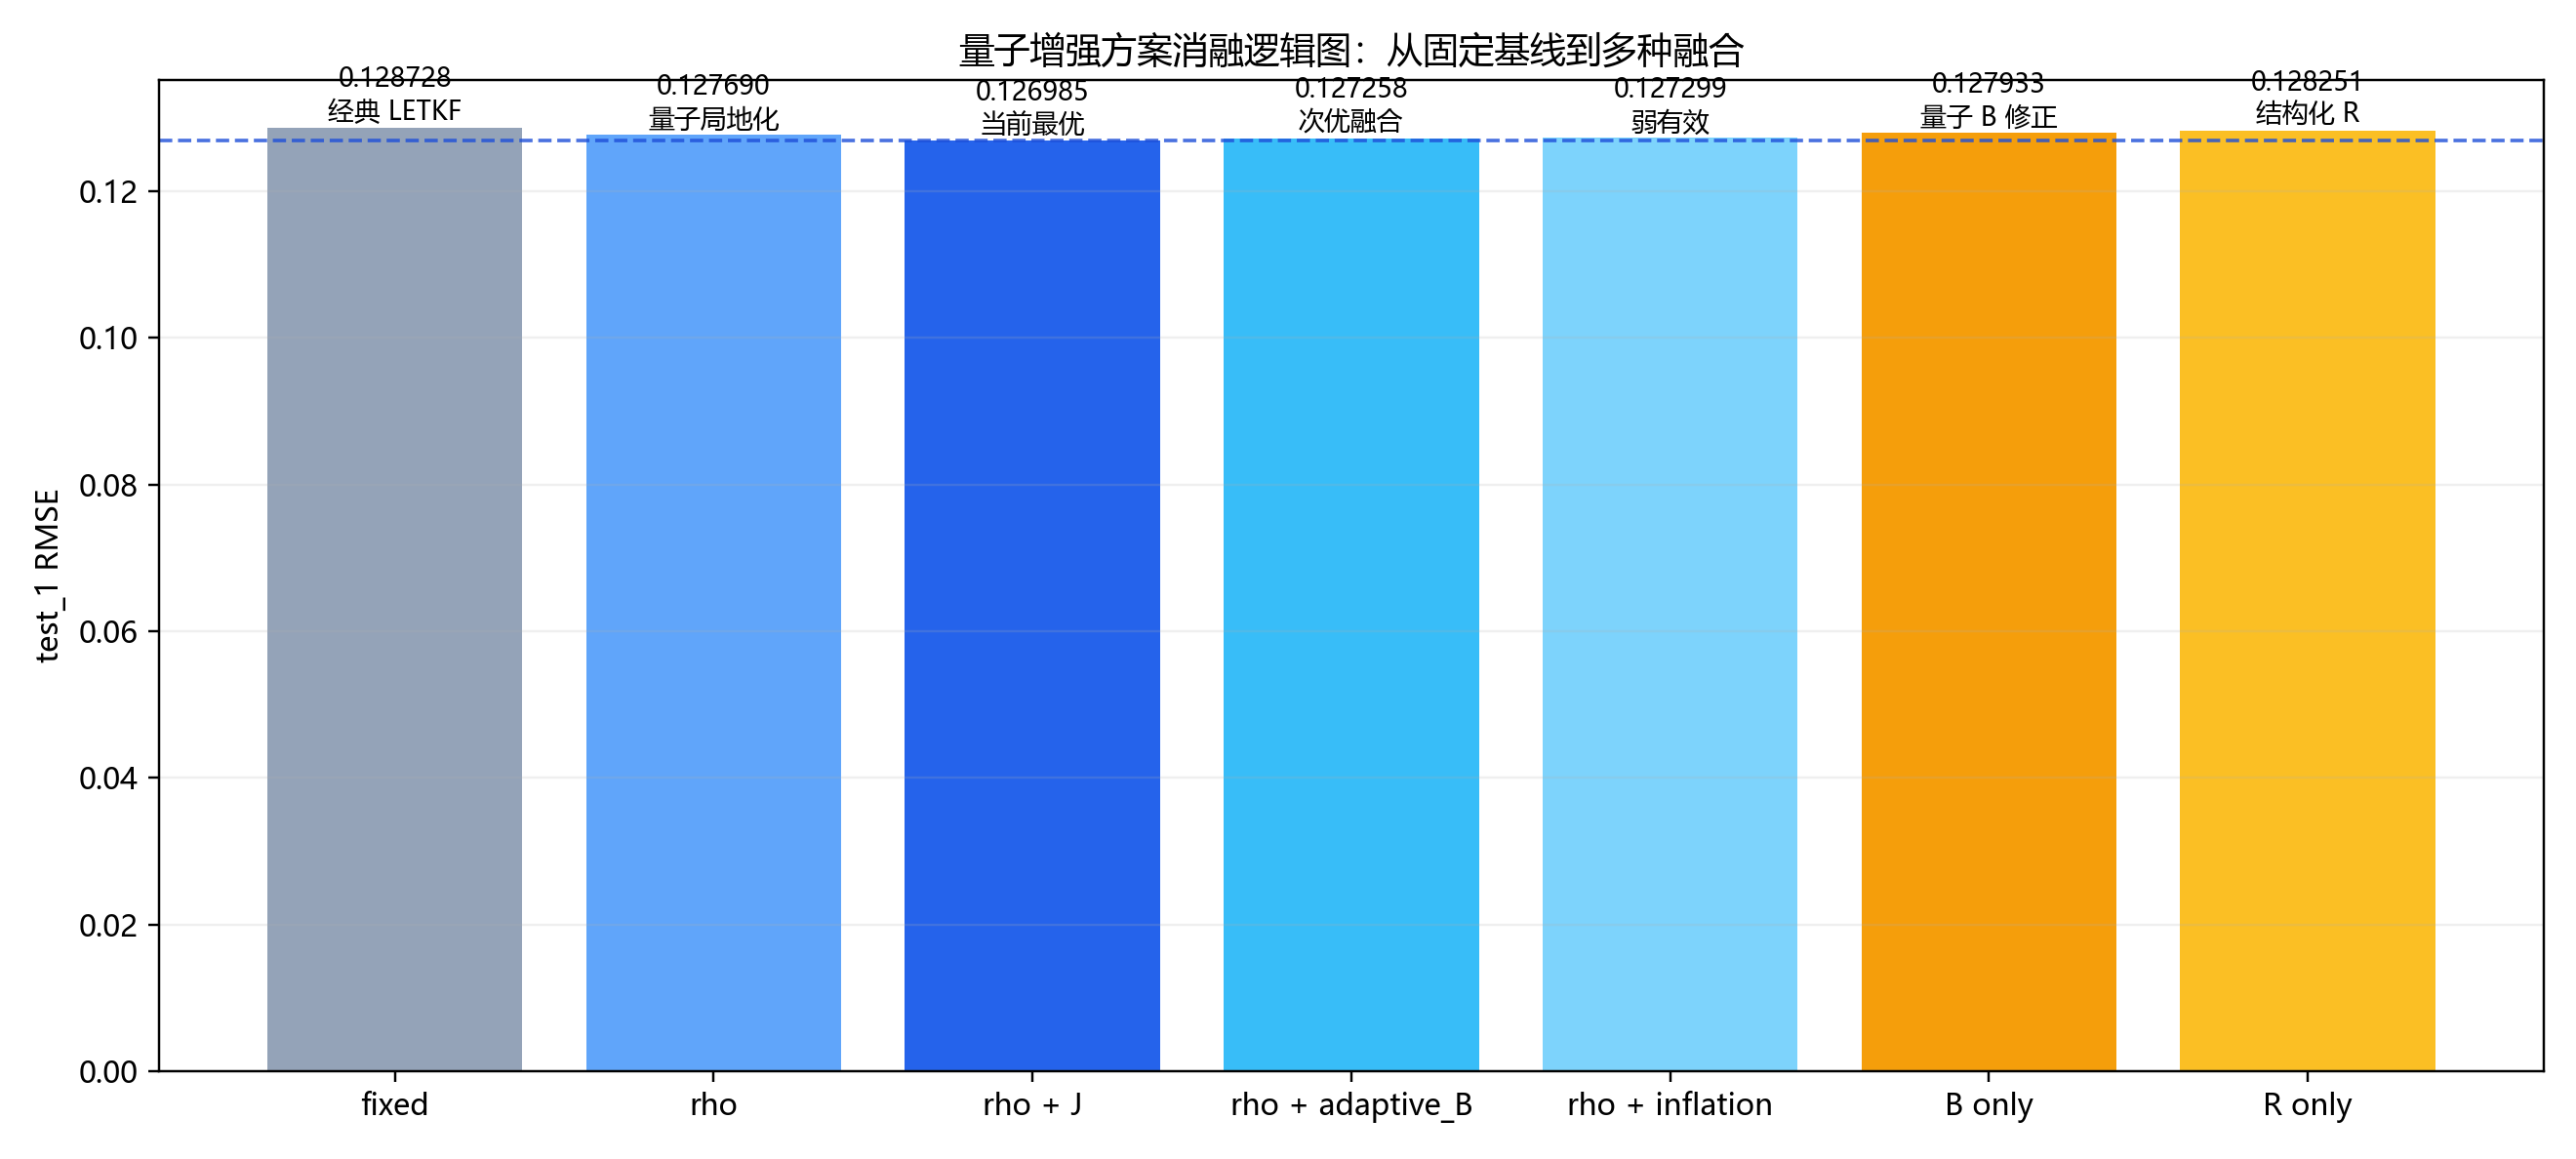
\includegraphics[width=0.92\linewidth]{figures/quantum_ablation_logic.png}
\caption{从经典基线到量子弱融合的整体消融逻辑。}
\label{fig:ablation}
\end{figure}

图 \ref{fig:ablation} 给出了本文的方法推进逻辑。可以看到，我们并不是从一开始就追求复杂的量子替代，而是从经典基线出发，逐步检验量子结构信息的作用位点，并在失败与修正中收敛到当前的弱融合主线。若没有这一步分层验证，量子模块很容易沦为形式化嵌入，既无法解释其作用，也无法稳定复现其收益。

更具体地说，这条推进链可以分成三个阶段。第一阶段是“结构验证”：先确认量子特征映射是否真的能在局地窗口上产生非平凡相似度，而不是随机噪声。第二阶段是“强接入试探”：尝试把量子结构更直接地注入同化权重，观察其是否能成为主导更新信号。第三阶段则是“弱融合收敛”：在确认强接入会退化后，重新设计量子模块的角色，让其只承担温和调制和小幅方向修正的任务。也正是在这一阶段，本文逐步形成了“距离先验保底、量子相似度补充、弱 $J$ 修正后置”的总体框架。

这条实验路线本身也是本文工作量和思考过程的重要组成部分。我们并不是一次性写出最终方案，而是在多轮实验中逐步回答三个问题：量子结构是否存在，量子结构如何进入公式，量子结构进入后为什么会成功或失败。前两个问题决定“能不能做”，第三个问题决定“怎么做才合理”。从最终文本结构上看，后续的建模、算法设计、实验结果和创新点描述，实际上都围绕这三个问题展开。

从论文叙事的角度看，图 \ref{fig:ablation} 的意义不只是展示做过哪些实验，而是说明本文的主线是一条“由失败推动问题收缩”的研究主线。直接接入失败并不是负面结果，恰恰是它告诉我们：量子信号并不适合强行充当主导权重，而更适合作为局地几何修正信号。基于当前受控实验，本文更适合被理解为一份“量子弱融合在 Lorenz96 上的机制验证报告”，而不是一篇已经完成大规模外推的方法论终稿。
